\bigskip

\item The graph below is a representation of which function?

% \resizebox{3in}{!}{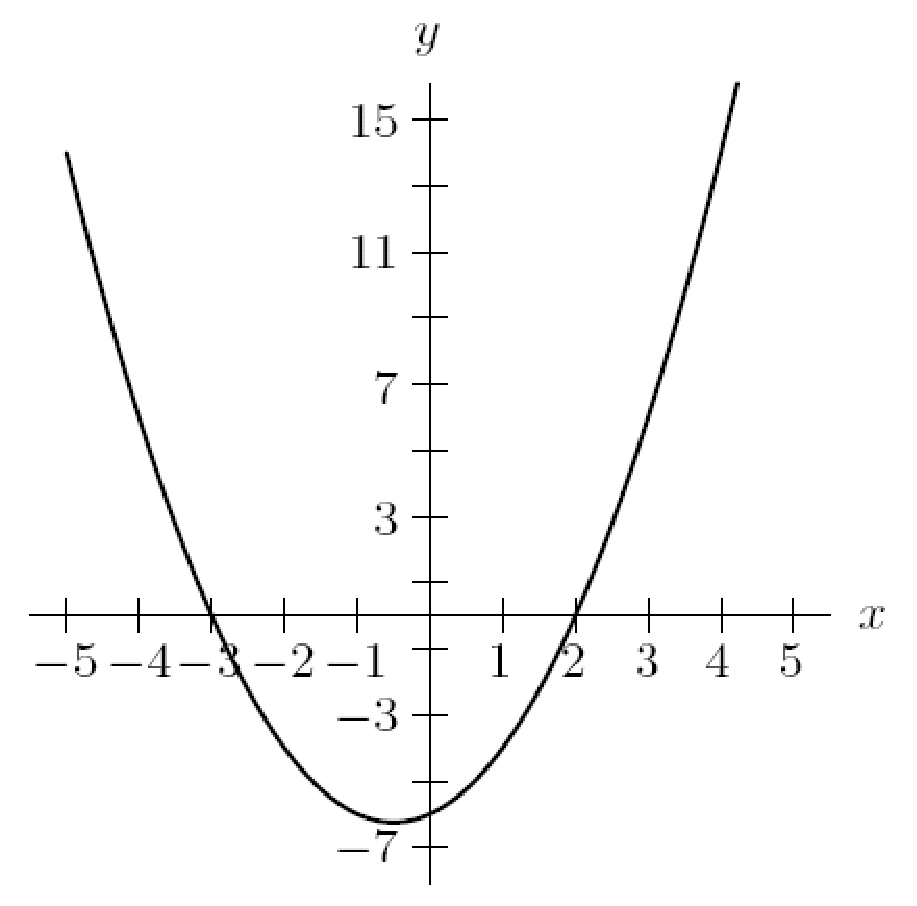
\includegraphics{SVC.01.06.090.ps}}

\begin{minipage}{0.4\columnwidth}
    \begin{enumerate}
        \item $y = 3x + 2$
        \item $y = (x-2)(x+3)$
        \item $y = (x-6)(x-2)$
        \item $y = (x-3)(x+2)$
        \item none of these
    \end{enumerate}
\end{minipage}
\begin{minipage}{0.6\columnwidth}
    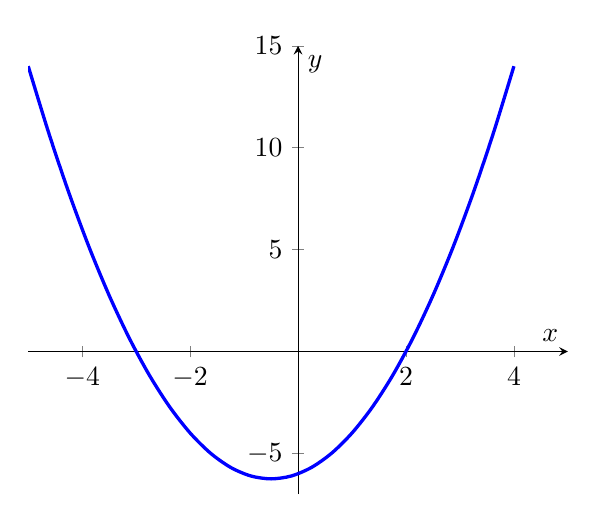
\begin{tikzpicture}
        \begin{axis}[axis lines=center, xlabel={$x$}, ylabel={$y$}, xmin=-5, xmax=5,
            ymin=-7, ymax=15]
            \addplot[color=blue, very thick, domain=-5:4, smooth]
            {(x+3)*(x-2)};
        \end{axis}
    \end{tikzpicture}
\end{minipage}

% ConcepTests - to accompany Calculus 4th Edition, Hughes-Hallet et al. John Wiley \& Sons.
